\chapter{What is software architecture ?}

The architecture of a software system is the shape given to that system by those
who build it. The form of that shape is in the division of that system into
components, the arrangement of those components, and the ways in which those
components communicate with each other. The purpose of that shape is to
facilitate the development, deployment, operation, and maintenance of the
software system contained within it.

\section{Goals of an architecture}

The software must change to adapt to software regulation, user feedback.

We have some pattern that make methods and classes easy to be changed, but now
we want something behond the methods.

The goals of an architecture are:
\begin{itemize}
  \item keep the system valuable for its users over time
  \item minimize the lifetime cost of the system
  \item maximize programmer productivity
\end{itemize}

This can be achieved by making the system:

\begin{itemize}
  \item easy to understand
  \item easy to develop
  \item easy to maintain
  \item easy to deploy
  \item easy to change
\end{itemize}

In Java we have the package, that is a module, and is a logical grouping of classes.


\begin{itemize}
  \item Design Patterns: helps to build methods and classes inside the module in a
        way that they are easy to be changed.
  \item Design Principles: define the modules can collaborate together and how they
        are shaped.
\end{itemize}

\section{The clear architectures}


\begin{itemize}
  \item Outer circles: mechanisms, they change often.
  \item Inner circles: policies, subject to less frequent changes
\end{itemize}


\begin{center}
  \begin{minipage}{\linewidth}
    % Primo blocco: 50% dello spazio per il codice
    \begin{minipage}{0.6\linewidth}
      Source code dependencies point only inward, toward higher-level policies
      (Dependency Rule)
    \end{minipage}% <-- IMPORTANTE: il simbolo % qui evita spazi bianchi extra
    \hfill % Spazio elastico automatico per distanziare i due blocchi
    % Secondo blocco: 40% dello spazio per l'immagine
    \begin{minipage}{0.40\linewidth}
      \centering
      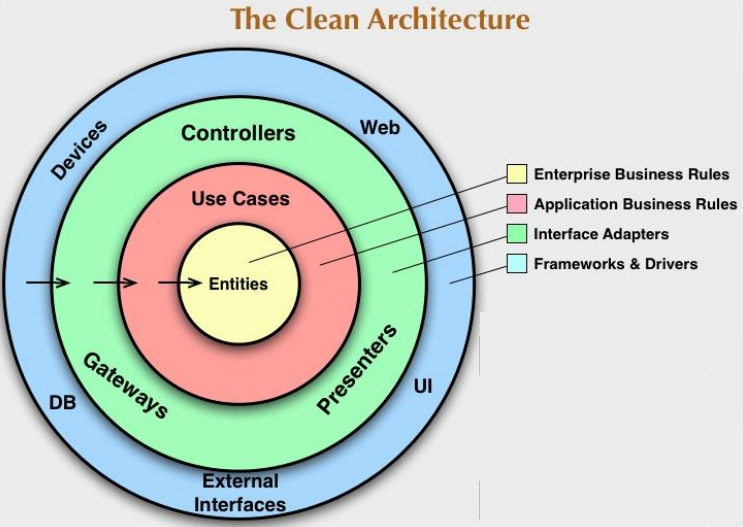
\includegraphics[width=\linewidth]{images/SA/SA-esempio1.png}
    \end{minipage}
  \end{minipage}
\end{center}

\subsection{Entities}

An Entity is an object within a software system that contains a set of critical
business rules operating on Critical Business Data.

\paragraph{Example:} The system is the university portal and an important entity is the student, that
has some critical business rules like "the student can enroll to the master degree only
if they have completed the required prerequisites and then assign new ID".

Is the most stable part of the system and we want to preserve as much as possible
from changes occurring to the other elements.



\begin{center}
  \begin{minipage}{\linewidth}
    % Primo blocco: 50% dello spazio per il codice
    \begin{minipage}{0.6\linewidth}
      The interface of the Entity consists of the functions that
      implement the Critical Business Rules to operate on the Critical
      Business Data.

      They contain the most general and highlevel rules and
      neither they are often changed nor they are usually affected by
      lower-level changes.
    \end{minipage}% <-- IMPORTANTE: il simbolo % qui evita spazi bianchi extra
    \hfill % Spazio elastico automatico per distanziare i due blocchi
    % Secondo blocco: 40% dello spazio per l'immagine
    \begin{minipage}{0.40\linewidth}
      \centering
      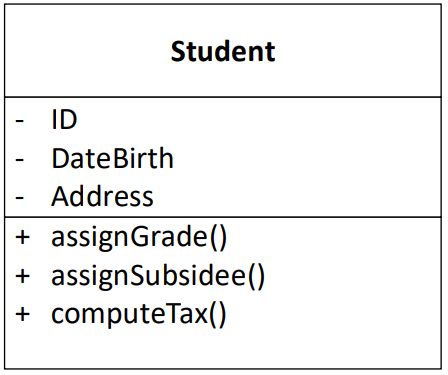
\includegraphics[width=\linewidth]{images/SA/SA-esempio2.png}
    \end{minipage}
  \end{minipage}
\end{center}

\section{Use cases}
To applay the Businness Roles to the entities we need to use the use cases.

A use case is a description of the software behavior and interactions (with
people or other software) in a specific case.

It specifies:

\begin{itemize}
  \item the input to be provided by the user (or other systems)
  \item the output to be returned
  \item The processing steps involved.
\end{itemize}

to determine the flow of data to and from the entities.

\subsubsection{Use case in pratice}
It represents a \textbf{functional requirement}.

\begin{itemize}
  \item It makes clear what you expect from a system ("what?")
  \item It hides the behaviour of the system ("how?")
  \item It is a sequence of actions (with variants) that produce a result observable by an actor
\end{itemize}

\begin{center}
  \begin{minipage}{\linewidth}
    \begin{minipage}{0.6\linewidth}
     The system is seen as a black-box. Use cases express the interaction
      (exchange of messages) between the entities that interact with the system
      itself (called actors).
    \end{minipage}% <-- IMPORTANTE: il simbolo % qui evita spazi bianchi extra
    \hfill
    \begin{minipage}{0.40\linewidth}
      \centering
      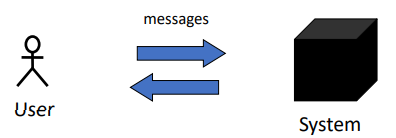
\includegraphics[width=\linewidth]{images/SA/SA-esempio3.png}
    \end{minipage}
  \end{minipage}
\end{center}




\paragraph{Example - Specify annual tax for a student}
Input: student ID\newline
Output: annual tax amount\newline

Main scenario:
\begin{enumerate}
  \item Validate ID provided by user
  \item Retrieve economic level
  \item Compute due past taxes
  \item Compute new taxes
  \item Get average grades for the last academic year
  \item If average grade > 26, apply 20\% discount
  \item Ask operator for confirmation: if yes change student else reset
\end{enumerate}


\section{Interface adapters}


\section{Frameworks and drivers}

In order to achieve the separation we have seen so far, we need to separate
low level details from the high-level details.

The details are the frameworks, the database, the drivers, the web server, etc., 
and usually we do not write mutch code here.


\section{Separation of policy from details}



\begin{center}
  \begin{minipage}{\linewidth}
    \begin{minipage}{0.6\linewidth}
    Decoupling of policy from the details and efer decisions on details for
     as long as possible (MongoDB or SQL, etc.)
    \end{minipage}% <-- IMPORTANTE: il simbolo % qui evita spazi bianchi extra
    \hfill
    \begin{minipage}{0.40\linewidth}
      \centering
      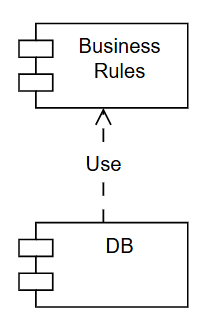
\includegraphics[width=\linewidth]{images/SA/SA-esempio5.png}
    \end{minipage}
  \end{minipage}
\end{center}



\begin{center}
  \begin{minipage}{\linewidth}
    \begin{minipage}{0.6\linewidth}
    The Database component contains the code that translates the calls made
    by the BusinessRules into the query language of the database. This
    translation code knows about the BusinessRules. 
    
    Business rules can be
    adapted to any kind of DB.
    \end{minipage}% <-- IMPORTANTE: il simbolo % qui evita spazi bianchi extra
    \hfill
    \begin{minipage}{0.40\linewidth}
      \centering
      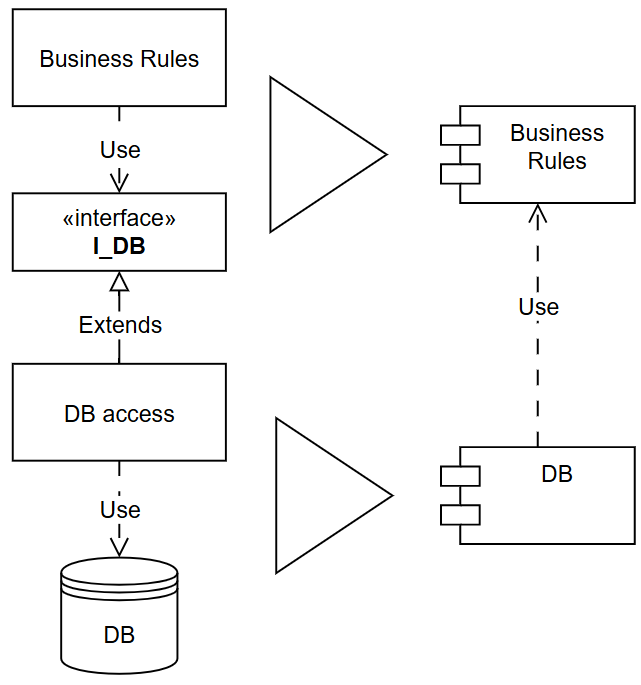
\includegraphics[width=\linewidth]{images/SA/SA-esempio4.png}
    \end{minipage}
  \end{minipage}
\end{center}






